% Imported from algorithms/audio-video-joint/README.md
\chapter{M05 音视频联合生成}\label{seedance-m05}
\moduleinfo{M05}{基础方法与机制解释}{\hyperref[src-seedance-1.5-pro]{\texttt{seedance-1.5-pro}}、\hyperref[src-seedance-2.0]{\texttt{seedance-2.0}}、\hyperref[src-seedance-2.5-release]{\texttt{seedance-2.5-release}}、\hyperref[src-ltx-code]{\texttt{ltx-code}}、\hyperref[src-ltx-2]{\texttt{ltx-2}}、\hyperref[src-ltx-original-code]{\texttt{ltx-original-code}}}


给一段视频配上声音，与从同一个事件同时生成画面和声音，是两种不同的任务。前者可以先完成画面，再制作对白、音乐和音效；后者需要模型在生成过程中同时考虑嘴形、语调、动作节奏和环境声。原生音视频联合生成的价值，正是让两种模态共同决定``发生了什么''。

\section{两个生成分支为什么仍要交换信息}\label{seedance-m05-ux4e24ux4e2aux751fux6210ux5206ux652fux4e3aux4ec0ux4e48ux4ecdux8981ux4ea4ux6362ux4fe1ux606f}

视频和音频的数据结构不同。视频潜变量保留时间、空间和通道，音频潜变量通常以一维时间序列为主。让两者各用适合自身结构的主干，再通过联合模块交换信息，是一种可行的双分支设计。

\[
z_v\in\mathbb{R}^{B\times C_v\times T_v\times H_v\times W_v},
\qquad
z_a\in\mathbb{R}^{B\times C_a\times T_a}.
\]

视频分支预测画面速度场，音频分支预测声音速度场，文本和参考为它们提供共同条件。Seedance 1.5 Pro 采用双分支 DiT 与跨模态联合模块，但具体 codec、插入层和连接公式需要按实现确定。

\begin{figure}
\centering
\pandocbounded{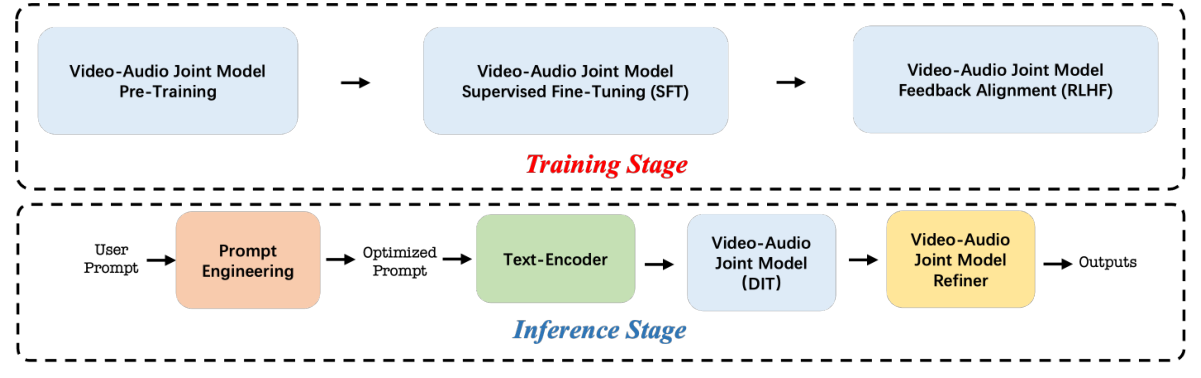
\includegraphics[keepaspectratio,alt={音视频模型的训练与生成流程 （论文示意，来源：seedance-1.5-pro）}]{assets/seedance/figures/audio-video-pipeline.png}}
\caption{音视频模型的训练与生成流程 （论文示意，来源：seedance-1.5-pro）}
\end{figure}

训练部分先学习联合分布，再用高质量样本和反馈优化；生成部分从提示改写、文本编码进入联合模型，必要时经过精修。图中呈现的是整体流程，不能用它代替具体交换模块的定义。

如果两个分支完全独立，即便输入同一个提示，也可能出现``画面里已经落地，声音还没响''或``人嘴闭着但仍在说话''。联合模块需要让一个模态读取另一个模态的当前生成状态。

\section{一种明确的交换方式}\label{seedance-m05-ux4e00ux79cdux660eux786eux7684ux4ea4ux6362ux65b9ux5f0f}

可以在部分层加入双向交叉注意力：

\[
\Delta h_v=\operatorname{Attn}(Q_v,K_a,V_a),
\qquad
\Delta h_a=\operatorname{Attn}(Q_a,K_v,V_v).
\]

再通过门控残差把增量加回各分支。这个公式是双分支方案的一种选择，并不意味着所有联合模型都采用相同结构。门控可以从零开始，使新模块在训练初期不干扰已有生成能力。

双向交换仍然有计算代价。若视频和音频 token 数分别为 \(N_v,N_a\)，一次完整交互的连接规模约为 \(N_vN_a\)。可以限制读取相近时间、先池化摘要，或者减少交换层，但每种压缩都会牺牲一部分对齐信息。

\section{同步依赖物理时间，不依赖相同索引}\label{seedance-m05-ux540cux6b65ux4f9dux8d56ux7269ux7406ux65f6ux95f4ux4e0dux4f9dux8d56ux76f8ux540cux7d22ux5f15}

假设视频为 24 fps，音频编码器每秒输出 50 个 token。两秒事件附近对应视频帧号 48、音频 token 号 100，它们的索引显然不能直接一一对应。还要考虑 VAE 时间压缩、音频 codec 的感受野、首帧规则和固定延迟。

可靠的做法是为每个 token 保存其覆盖的物理时间区间，并统一时间起点。局部跨模态 attention 才能按照``相隔多少毫秒''建立邻域，而不是按两个不相容的 token 序号建立邻域。

数据预处理也必须真正重采样。修改采样率或 fps 的元数据不会自动改变波形和帧序列；错误的时间戳会把输入错位变成模型必须学习的噪声。

\section{一套具体的共同表示}\label{seedance-m05-ux4e00ux5957ux5177ux4f53ux7684ux5171ux540cux8868ux793a}

LTX-2原系列提供了可参照的完整表示：视频latent为128通道，时间压缩8倍、空间各32倍；音频codec可保留 \codepath{B,8,Ta,16}，再展平为每时间位置128维，约25个时间位置/秒。音频输入使用16kHz的mel表示，经vocoder输出24kHz立体声；采样率与latent时间率是不同量。

这些配置应与同一系列的文本、归一化、调制和scheduler配套。视频压缩首帧规则要求内部帧数满足 \(F=1+8k\)，音频时长则按共同媒体时钟处理。采用这类现成联合主干后，新任务主要增加参考与源条件接口；无需再假设任意视频latent都能直接与一个音频生成器相接。

\section{两种损失怎样配平}\label{seedance-m05-ux4e24ux79cdux635fux5931ux600eux6837ux914dux5e73}

令噪声时间 \(t=0\) 对应数据、\(t=1\) 对应噪声。一种基础联合目标为：

\[
\mathcal{L}=\lambda_v\operatorname{MSE}(u_v,\epsilon_v-z_v)
+\lambda_a\operatorname{MSE}(u_a,\epsilon_a-z_a).
\]

两项应先分别按有效元素归一化，再观察损失量级与梯度范数。简单地把所有元素求和，会让 token 更多或数值尺度更大的模态主导更新。权重也不能只根据通道数决定。

混合训练中，缺少音轨与真实静音必须分开。缺音轨样本不计算音频目标损失；静音样本则有有效的音频目标。若把缺失音频统一当成静音，就会教模型在有声事件中保持安静。对白、环境音和音乐也应分别描述，画面中无法判断的台词不能被自动补成事实。

\section{怎样判断联合生成是否值得}\label{seedance-m05-ux600eux6837ux5224ux65adux8054ux5408ux751fux6210ux662fux5426ux503cux5f97}

口型、敲击、落地和脚步可以分别测量视觉事件与声音起点的偏差，单位统一为毫秒，同时人工复听语言、音色和情绪。同步分数之外，还要检查联合训练是否损伤画面的动作幅度或文本遵循，以及音频是否出现失真、杂音和无关音乐。

如果业务主要使用旁白，视频生成后配音和确定性混流往往已经可用。人物对白、唱歌和精确动作音效对联合建模的收益更大，但也需要更干净的对齐数据。是否增加音频分支，应由这些具体任务的质量与成本决定。

\section{从极简代码到真实实现}\label{seedance-m05-ux4eceux6781ux7b80ux4ee3ux7801ux5230ux771fux5b9eux5b9eux73b0}

双向交互需要两边都读取更新前的状态，否则执行顺序本身会引入不对称：

\begin{verbatim}
delta_video = attention(video_q, audio_k, audio_v)
delta_audio = attention(audio_q, video_k, video_v)
new_video = video + delta_video
new_audio = audio + delta_audio
\end{verbatim}

单头教学版本见 \hyperref[code-audio-video-exchange]{audio\_video\_exchange.py}；真实联合模块可读 \href{https://github.com/Lightricks/LTX-2/blob/daa6b16fc7f0f1628f2c9e36a303e3312b333cc6/packages/ltx-core/src/ltx_core/model/transformer/transformer.py}{LTX 的 BasicAVTransformerBlock}。它包含自己的调制、位置和条件接口，应作为独立音视频工程阅读，而不是直接当作 Wan 的音频插件。
